\documentclass[11pt]{article}

\usepackage[a4paper,margin=1in]{geometry}
\usepackage{amsmath,amssymb}
\usepackage{fontspec}
\usepackage{xeCJK}
\usepackage{xcolor}
\usepackage{hyperref}
\usepackage{booktabs}
\usepackage{longtable}
\usepackage{array}
\usepackage{seqsplit}
\usepackage{enumitem}
\usepackage{listings}
\usepackage[most]{tcolorbox}
\usepackage{titlesec}
\usepackage{fancyhdr}
\usepackage{parskip}
\usepackage{tikz}
\usetikzlibrary{arrows.meta,positioning,fit,shapes.geometric}

\IfFontExistsTF{PingFang SC}{\setCJKmainfont{PingFang SC}}{\setCJKmainfont{Songti SC}}
\setmainfont{Helvetica Neue}
\setmonofont{Menlo}

\definecolor{axonblue}{HTML}{1F4E79}
\definecolor{axongray}{HTML}{4A5568}
\definecolor{axonlight}{HTML}{F6F8FA}
\definecolor{axonred}{HTML}{9B1C1C}
\definecolor{axongreen}{HTML}{166534}
\definecolor{axonamber}{HTML}{92400E}

\hypersetup{
  colorlinks=true,
  linkcolor=axonblue,
  urlcolor=axonblue,
  citecolor=axonblue
}

\pagestyle{fancy}
\setlength{\headheight}{14pt}
\fancyhf{}
\lhead{EasyNet 状态机器}
\rhead{2026-06-09}
\cfoot{\thepage}

\titleformat{\section}{\Large\bfseries\color{axonblue}}{\thesection}{0.6em}{}
\titleformat{\subsection}{\large\bfseries\color{axongray}}{\thesubsection}{0.6em}{}

\newcommand{\tagaxiom}{\textcolor{axonblue}{\texttt{[axiom]}}}
\newcommand{\tagderived}{\textcolor{axongreen}{\texttt{[derived]}}}
\newcommand{\tagdeferred}{\textcolor{axonamber}{\texttt{[deferred]}}}
\newcommand{\code}[1]{\texttt{#1}}
\newcommand{\statecode}[1]{{\ttfamily\scriptsize\seqsplit{#1}}}

\newcolumntype{L}[1]{>{\raggedright\arraybackslash}p{#1}}

\newtcolorbox{invariantbox}{
  colback=axonlight,
  colframe=axonblue,
  title=Invariant,
  fonttitle=\bfseries,
  arc=2mm
}

\newtcolorbox{decisionbox}{
  colback=white,
  colframe=axongreen,
  title=Decision,
  fonttitle=\bfseries,
  arc=2mm
}

\newtcolorbox{warningbox}{
  colback=white,
  colframe=axonred,
  title=Failure Contract,
  fonttitle=\bfseries,
  arc=2mm
}

\lstdefinestyle{easynet}{
  basicstyle=\ttfamily\small,
  backgroundcolor=\color{axonlight},
  frame=single,
  rulecolor=\color{axongray},
  breaklines=true,
  columns=fullflexible
}
\lstdefinelanguage{json}{
  basicstyle=\ttfamily\small,
  showstringspaces=false,
  breaklines=true,
  morestring=[b]",
  stringstyle=\color{axonblue},
  literate=
   *{0}{{{\color{axonred}0}}}{1}
    {1}{{{\color{axonred}1}}}{1}
    {2}{{{\color{axonred}2}}}{1}
    {3}{{{\color{axonred}3}}}{1}
    {4}{{{\color{axonred}4}}}{1}
    {5}{{{\color{axonred}5}}}{1}
    {6}{{{\color{axonred}6}}}{1}
    {7}{{{\color{axonred}7}}}{1}
    {8}{{{\color{axonred}8}}}{1}
    {9}{{{\color{axonred}9}}}{1}
    {:}{{{\color{axongray}{:}}}}{1}
    {,}{{{\color{axongray}{,}}}}{1}
    {\{}{{{\color{axongray}{\{}}}}{1}
    {\}}{{{\color{axongray}{\}}}}}{1}
    {[}{{{\color{axongray}{[}}}}{1}
    {]}{{{\color{axongray}{]}}}}{1}
}
\lstset{style=easynet}
\emergencystretch=2em

\tikzset{
  state/.style={rectangle,rounded corners=2mm,draw=axonblue,fill=axonlight,align=center,minimum width=2.9cm,minimum height=0.9cm,font=\small},
  fail/.style={rectangle,rounded corners=2mm,draw=axonred,fill=white,align=center,minimum width=2.9cm,minimum height=0.9cm,font=\small},
  edge/.style={-{Latex[length=2mm]},thick,draw=axongray},
  dashededge/.style={-{Latex[length=2mm]},thick,dashed,draw=axongray}
}

\title{\textbf{EasyNet 状态机器完整设计}\\
\large Join、Resolve、Invoke、Read Model 与 Failure 可追踪契约}
\author{EasyNet Engineering}
\date{2026-06-09}

\begin{document}
\maketitle

\begin{abstract}
本文定义 EasyNet 从前端 pairing token 到 \code{easynet join}、CLI daemon 接入 Hub/Axon runtime、Backend/Frontend 显示 connected 的完整状态机器, 同时覆盖 RFC-005 URA namespace resolution 迁移后的 ability resolve、invoke、read model 和 failure propagation。核心目标是: 每个用户可见状态都有稳定状态码; 每个失败都能定位到具体 transition; 所有 invocation 必须先经过 Axon \code{ResolveAnswer.FinalRoute}, 再按 resolver-selected next hop dispatch。
\end{abstract}

\tableofcontents
\newpage

\section{结论}

\begin{invariantbox}
\tagaxiom{} \code{credential accepted != daemon connected != namespace visible != frontend connected}。
\end{invariantbox}

\begin{invariantbox}
\tagaxiom{} bare ability name 只能作为 resolver query input。Backend prepare、Frontend signing、CLI daemon dispatch 和 signed Invocation 必须使用 \code{ResolveAnswer.FinalRoute} 中的 canonical \code{ability\_ura}、\code{route\_ura}、\code{dispatch\_name} 和 \code{next\_hop}。
\end{invariantbox}

当前问题不是单一 HTTP 页面、单一 ability 或单一 handler 的 bug, 而是 RFC-005 迁移尚未完全收敛后的系统性状态机器缺口。症状包括: join 保存 credential 后 daemon 连接失败却曾被当作成功; \code{terminal.list} 因 device 不在 PresenceRegistry 返回 fallback; \code{pages.list} 因 agent 未 advertised 变成普通 500; \code{history/list} 因缺 canonical route 返回裸 400; \code{meta.list\_resources} 缺 resolver catalog route。

\section{仓库边界}

\begin{longtable}{L{0.20\linewidth} L{0.36\linewidth} L{0.36\linewidth}}
\toprule
层 & 应拥有 & 不应拥有 \\
\midrule
EasyNet-Axon & URA 语法、\code{ResolveQuery}、\code{ResolveAnswer}、route evidence、negative taxonomy、failure code、\code{InvocationReceipt.failure} & Backend 产品 DB、Frontend UX、CLI 本地插件实现 \\
EasyNet-Cli daemon & local device abilities、hosted agent runtime、Axon bridge/session、device namespace authority、resolve-before-invoke、local receipt producer & Backend HTTP policy、Frontend connected 判定 \\
EasyNet Backend & pairing lifecycle、credential issuance、user ownership、read model projection、typed unavailable DTO、signed invoke prepare/submit facade & URA canonicalization fork、owner/route inference、Axon resolver negative 字符串解析 \\
EasyNet Frontend & token UX、SSE cache invalidation、typed state rendering、actionable error display & liveness truth、ability route builder、resolver fallback \\
\bottomrule
\end{longtable}

\begin{decisionbox}
\tagderived{} Backend 经 daemon.sock 调 Hub/daemon ability 是合法 transport-binding; Backend 在 Go 里 fork Axon 协议契约是不合格实现。Frontend 只能消费 API routes/read model, 不能拼 canonical ability URA。
\end{decisionbox}

\section{状态码规则}

\begin{longtable}{L{0.12\linewidth} L{0.72\linewidth}}
\toprule
前缀 & 语义 \\
\midrule
\code{P} & Pairing token lifecycle \\
\code{J} & Join credential lifecycle \\
\code{S} & Session/runtime lifecycle \\
\code{N} & Namespace visibility/readiness \\
\code{C} & Frontend connected/degraded UI \\
\code{R} & Resolver route selection \\
\code{I} & Invocation prepare/submit/execution \\
\code{M} & Mission/EAL composite invocation orchestration \\
\code{D} & Download/body-committed stream lifecycle \\
\code{O} & Operator runtime stop lifecycle \\
\code{U} & Self-uninstall/leave lifecycle \\
\code{A} & Ability catalog/read model \\
\code{F} & Failure terminal or degraded state \\
\bottomrule
\end{longtable}

状态码必须稳定、可定位、可追踪、可组合。稳定表示 UI、CLI、日志、测试不得依赖人类字符串。可定位表示 failure 必须携带 \code{transition}、\code{from\_state}、\code{interrupted\_state}。可组合表示列表 API 可以返回 product rows, 同时携带 \code{resolve\_unavailable[]}。

\section{Join 到 Connected 状态机器}

\subsection{状态图}

\begin{center}
\resizebox{\linewidth}{!}{
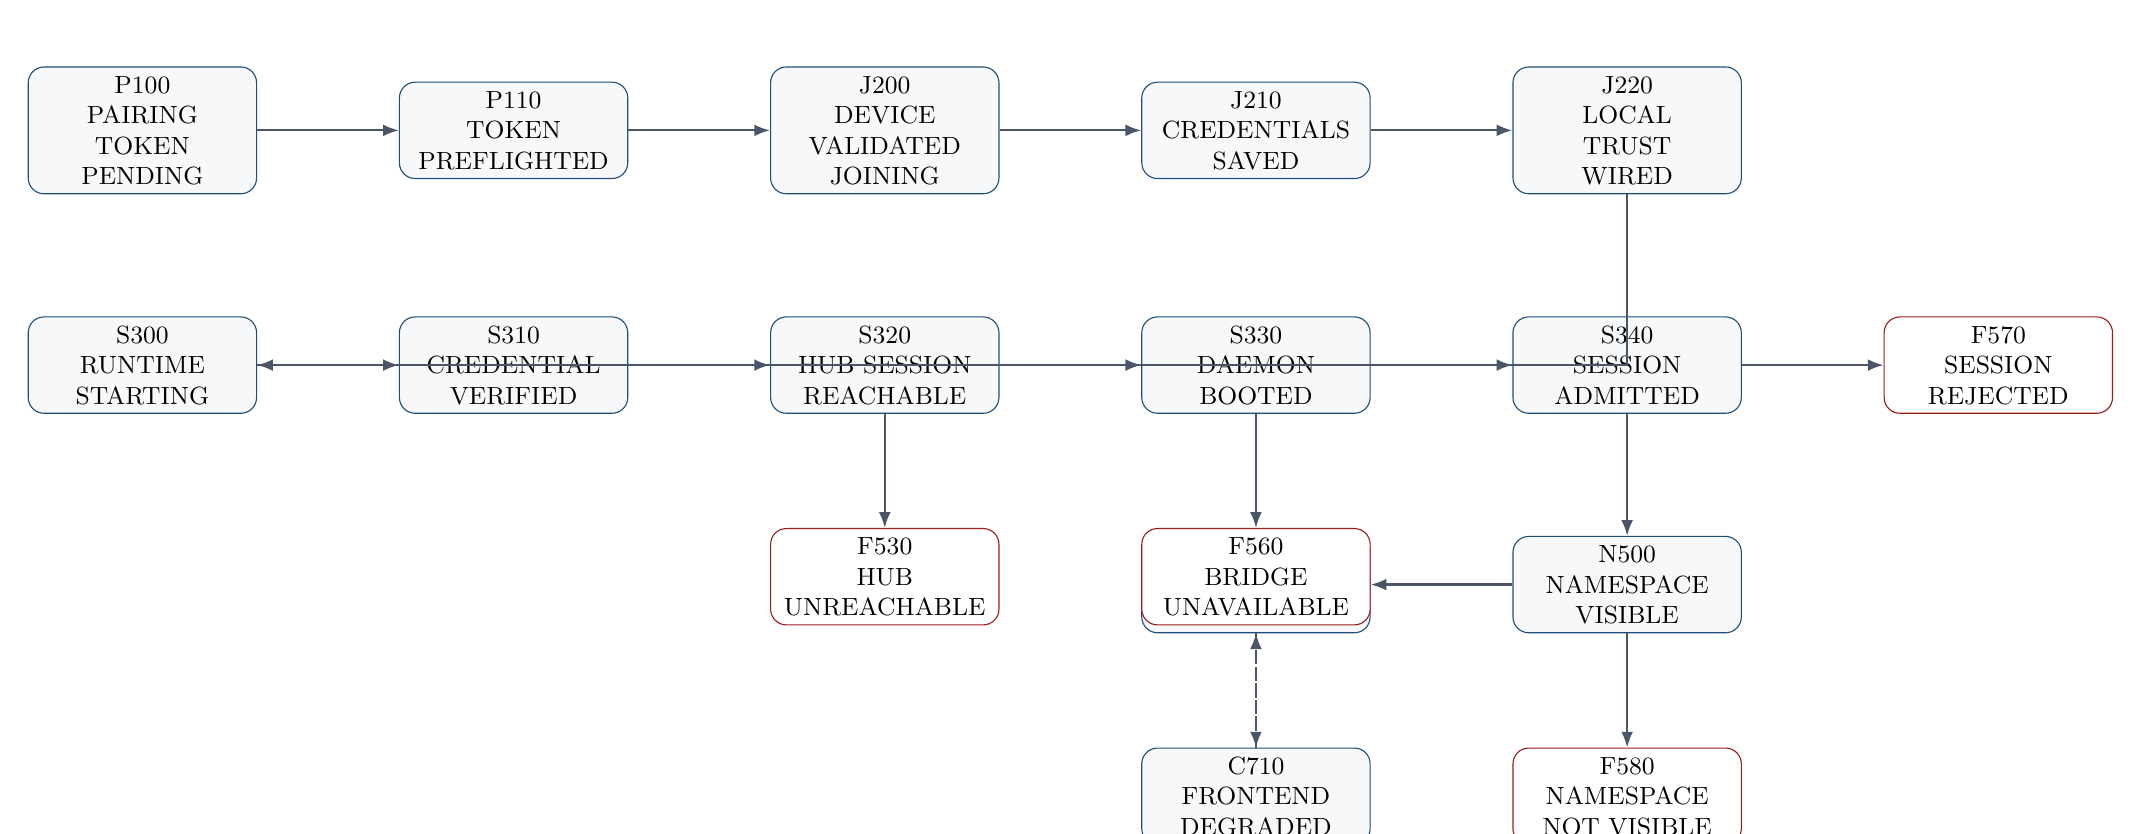
\begin{tikzpicture}[node distance=1.45cm and 1.8cm]
\node[state] (p100) {P100\\PAIRING\\TOKEN\\PENDING};
\node[state,right=of p100] (p110) {P110\\TOKEN\\PREFLIGHTED};
\node[state,right=of p110] (j200) {J200\\DEVICE\\VALIDATED\\JOINING};
\node[state,right=of j200] (j210) {J210\\CREDENTIALS\\SAVED};
\node[state,right=of j210] (j220) {J220\\LOCAL\\TRUST\\WIRED};
\node[state,below=1.55cm of p100] (s300) {S300\\RUNTIME\\STARTING};
\node[state,right=of s300] (s310) {S310\\CREDENTIAL\\VERIFIED};
\node[state,right=of s310] (s320) {S320\\HUB SESSION\\REACHABLE};
\node[state,right=of s320] (s330) {S330\\DAEMON\\BOOTED};
\node[state,right=of s330] (s340) {S340\\SESSION\\ADMITTED};
\node[state,below=1.55cm of s340] (n500) {N500\\NAMESPACE\\VISIBLE};
\node[state,left=of n500] (c700) {C700\\FRONTEND\\CONNECTED};
\node[state,below=of c700] (c710) {C710\\FRONTEND\\DEGRADED};
\node[fail,below=of s320] (f530) {F530\\HUB\\UNREACHABLE};
\node[fail,below=of s330] (f560) {F560\\BRIDGE\\UNAVAILABLE};
\node[fail,right=of s340] (f570) {F570\\SESSION\\REJECTED};
\node[fail,below=of n500] (f580) {F580\\NAMESPACE\\NOT VISIBLE};
\draw[edge] (p100) -- (p110);
\draw[edge] (p110) -- (j200);
\draw[edge] (j200) -- (j210);
\draw[edge] (j210) -- (j220);
\draw[edge] (j220) |- (s300);
\draw[edge] (s300) -- (s310);
\draw[edge] (s310) -- (s320);
\draw[edge] (s320) -- (s330);
\draw[edge] (s330) -- (s340);
\draw[edge] (s340) -- (n500);
\draw[edge] (n500) -- (c700);
\draw[dashededge] (c700) -- (c710);
\draw[dashededge] (c710) -- (c700);
\draw[edge] (s320) -- (f530);
\draw[edge] (s330) -- (f560);
\draw[edge] (s340) -- (f570);
\draw[edge] (n500) -- (f580);
\end{tikzpicture}
}
\end{center}

\subsection{状态表}

\begin{longtable}{L{0.10\linewidth} L{0.22\linewidth} L{0.18\linewidth} L{0.36\linewidth} L{0.08\linewidth}}
\toprule
Code & State & Owner & Meaning & Terminal \\
\midrule
\code{P100} & \statecode{PAIRING\_TOKEN\_PENDING} & Backend & token 已创建, hash 已保存, TTL 生效 & No \\
\code{P110} & \statecode{PAIRING\_TOKEN\_PREFLIGHTED} & Backend / CLI & CLI 证明持有 token, 取得 reserved node/trust material & No \\
\code{F120} & \statecode{PAIRING\_TOKEN\_EXPIRED} & Backend & token 过期 & Yes \\
\code{F130} & \statecode{PAIRING\_TOKEN\_CONSUMED} & Backend & token 已被使用或状态非 pending & Yes \\
\code{J200} & \statecode{DEVICE\_VALIDATED\_JOINING} & Backend & credential issued, DB 状态 validated, liveness 未证明 & No \\
\code{J210} & \statecode{CREDENTIALS\_SAVED} & CLI & credential/config/key material 已落本地 & No \\
\code{J220} & \statecode{LOCAL\_TRUST\_WIRED} & CLI & realm trust 和 federation peer 写入完成 & No \\
\code{S300} & \statecode{RUNTIME\_STARTING} & CLI & 正在启动 daemon & No \\
\code{S310} & \statecode{HUB\_CREDENTIAL\_VERIFIED} & CLI / Backend & Backend 接受 credential token & No \\
\code{S320} & \statecode{HUB\_SESSION\_ENDPOINT\_REACHABLE} & CLI & Hub session endpoint TCP/TLS 可达 & No \\
\code{S330} & \statecode{DAEMON\_BOOTED} & CLI & daemon.sock up, runtime process alive & No \\
\code{S340} & \statecode{SESSION\_ADMITTED} & CLI daemon / Hub & \code{session.open} admission 成功 & No \\
\code{N500} & \statecode{NAMESPACE\_VISIBLE} & Axon / Hub / CLI & device URA 已进入 resolver / PresenceRegistry 可见面 & No \\
\code{C700} & \statecode{FRONTEND\_CONNECTED} & Backend / Frontend & 后端 read model 投影 ONLINE, 前端显示 connected & No \\
\code{C710} & \statecode{FRONTEND\_DEGRADED} & Backend / Frontend & DB row 可显示, runtime resolver 有 typed unavailable & No \\
\code{C790} & \statecode{FRONTEND\_OFFLINE} & Backend / Frontend & session/heartbeat lost, 或 PresenceRegistry 不含该 device & No \\
\bottomrule
\end{longtable}

\subsection{Failure 表}

\begin{longtable}{L{0.09\linewidth} L{0.18\linewidth} L{0.21\linewidth} L{0.19\linewidth} L{0.25\linewidth}}
\toprule
Code & Failure & Interrupted transition & Source & Operator action \\
\midrule
\code{F530} & \statecode{HUB\_UNREACHABLE} & \code{S310 -> S320} & CLI socket preflight & 检查 Hub TLS endpoint, port, trust, compose \\
\code{F541} & \statecode{CREDENTIAL\_REJECTED} & \code{S300 -> S310} & Backend credential verify & 重新 join 或刷新 credential \\
\code{F550} & \statecode{DAEMON\_BOOT\_FAILED} & \code{S300 -> S330} & CLI daemon supervisor & 看 daemon log \\
\code{F560} & \statecode{BRIDGE\_UNAVAILABLE} & \code{S330 -> S340} & CLI Axon bridge loader & 设置 \statecode{EASYNET\_DENDRITE\_BRIDGE\_LIB/HOME} \\
\code{F570} & \statecode{SESSION\_ADMISSION\_REJECTED} & \code{S340 admission} & Hub admission / Axon & 检查 caller signature, trusted key, realm trust \\
\code{F580} & \statecode{NAMESPACE\_NOT\_VISIBLE} & \code{S340 -> N500} & resolver / PresenceRegistry & 检查 session 是否真的 admitted \\
\bottomrule
\end{longtable}

\begin{warningbox}
用户给出的 bridge missing 错误应记录为 \code{F560 BRIDGE\_UNAVAILABLE}, interrupted transition 是 \code{S330\_DAEMON\_BOOTED -> S340\_SESSION\_ADMITTED}, 而不是 join 成功。
\end{warningbox}

\section{Resolve / Invoke 状态机器}

\subsection{状态图}

\begin{center}
\resizebox{\linewidth}{!}{
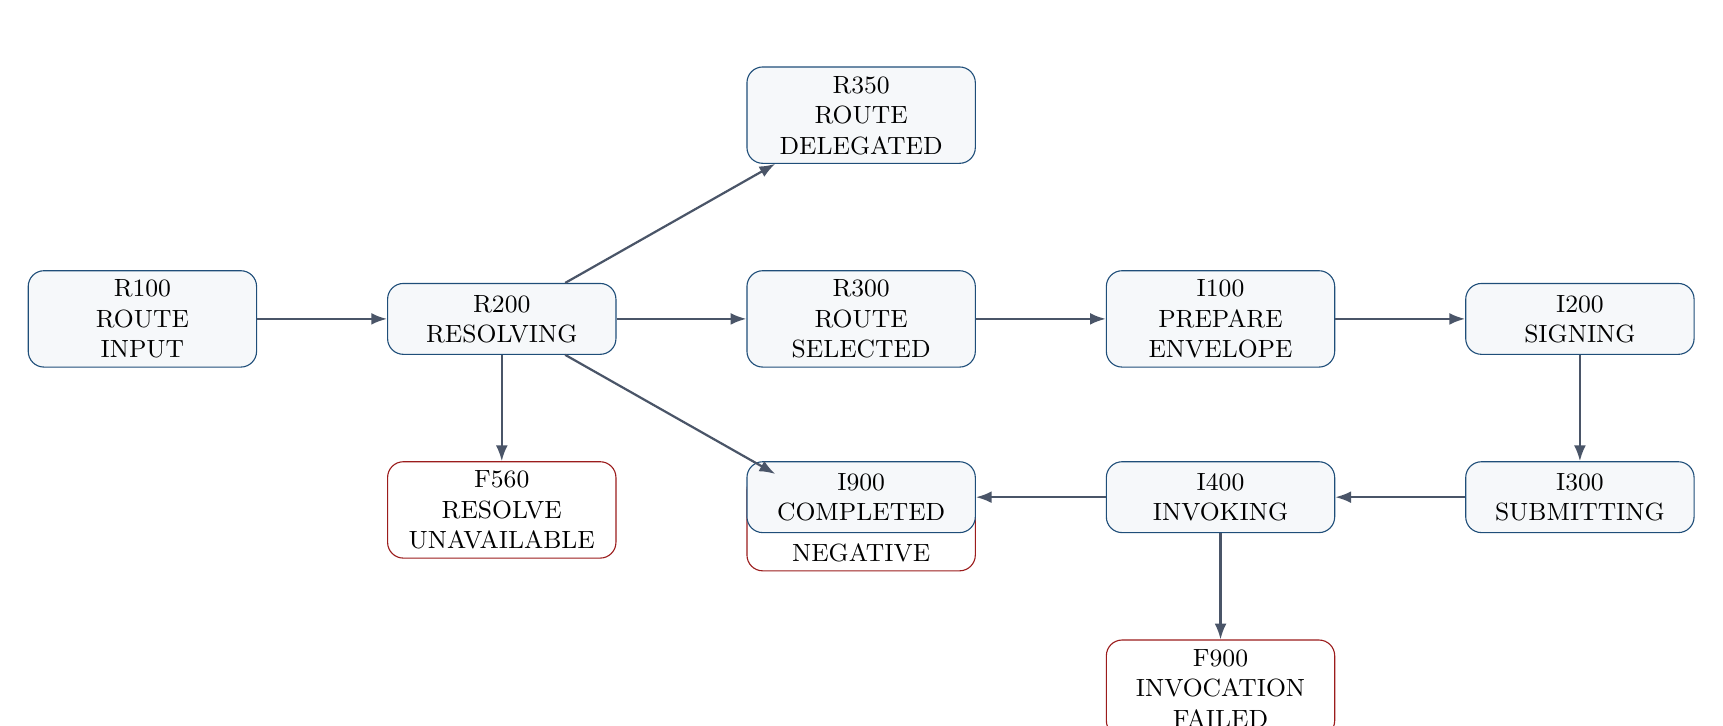
\begin{tikzpicture}[node distance=1.35cm and 1.65cm]
\node[state] (r100) {R100\\ROUTE\\INPUT};
\node[state,right=of r100] (r200) {R200\\RESOLVING};
\node[state,right=of r200] (r300) {R300\\ROUTE\\SELECTED};
\node[state,above=of r300] (r350) {R350\\ROUTE\\DELEGATED};
\node[fail,below=of r300] (r400) {R400\\ROUTE\\NEGATIVE};
\node[state,right=of r300] (i100) {I100\\PREPARE\\ENVELOPE};
\node[state,right=of i100] (i200) {I200\\SIGNING};
\node[state,below=of i200] (i300) {I300\\SUBMITTING};
\node[state,left=of i300] (i400) {I400\\INVOKING};
\node[state,left=of i400] (i900) {I900\\COMPLETED};
\node[fail,below=of i400] (f900) {F900\\INVOCATION\\FAILED};
\node[fail,below=of r200] (f560) {F560\\RESOLVE\\UNAVAILABLE};
\draw[edge] (r100) -- (r200);
\draw[edge] (r200) -- (r300);
\draw[edge] (r200) -- (r350);
\draw[edge] (r200) -- (r400);
\draw[edge] (r200) -- (f560);
\draw[edge] (r300) -- (i100);
\draw[edge] (i100) -- (i200);
\draw[edge] (i200) -- (i300);
\draw[edge] (i300) -- (i400);
\draw[edge] (i400) -- (i900);
\draw[edge] (i400) -- (f900);
\end{tikzpicture}
}
\end{center}

\subsection{Resolve 状态表}

\begin{longtable}{L{0.10\linewidth} L{0.18\linewidth} L{0.17\linewidth} L{0.43\linewidth}}
\toprule
Code & State & Owner & Required data \\
\midrule
\code{R100} & \statecode{ROUTE\_INPUT} & Backend / Frontend / CLI caller & \code{target\_ura}, \code{ability\_name}, \code{caller}, \code{subject}, \code{scope} \\
\code{R200} & \statecode{RESOLVING} & CLI daemon / Axon & normalized \code{ResolveQuery} \\
\code{R210} & \statecode{RESOLVING\_PEER} & Hub / Axon peer & delegation proof, authoritative realm \\
\code{R300} & \statecode{ROUTE\_SELECTED} & Axon & \code{ResolveAnswer.FinalRoute} with selected next hop \\
\code{R350} & \statecode{ROUTE\_DELEGATED} & Axon & peer hub delegation, no local dispatch \\
\code{R400} & \statecode{ROUTE\_NEGATIVE} & Axon & \code{NegativeReason}, code, retry policy \\
\code{F560} & \statecode{RESOLVE\_UNAVAILABLE} & CLI / Backend & transport/runtime failure locator \\
\bottomrule
\end{longtable}

\subsection{Invocation 状态表}

\begin{longtable}{L{0.10\linewidth} L{0.22\linewidth} L{0.18\linewidth} L{0.38\linewidth}}
\toprule
Code & State & Owner & Invariant \\
\midrule
\code{I100} & \statecode{PREPARING\_ENVELOPE} & Backend & 只能使用 \code{R300.selected\_route.ability\_ura} \\
\code{I200} & \statecode{SIGNING} & Frontend / client key & 签名输入必须是 backend prepared canonical envelope \\
\code{I300} & \statecode{SUBMITTING} & Backend & submit body 必须携带 selected route/evidence \\
\code{I400} & \statecode{INVOKING} & CLI daemon / Axon runtime & dispatch only with resolver-selected next hop \\
\code{I900} & \statecode{COMPLETED} & Runtime producer & \code{InvocationReceipt.state=Completed}, 不带 failure \\
\code{F900} & \statecode{INVOCATION\_FAILED} & Runtime producer & \code{InvocationReceipt.failure} 必须 populated \\
\code{F901} & \statecode{INVOCATION\_TIMED\_OUT} & Runtime producer & timeout reason 写入 typed failure \\
\code{F902} & \statecode{INVOCATION\_CANCELLED} & Runtime producer & cancellation reason 写入 typed failure \\
\bottomrule
\end{longtable}

\section{Ability Catalog / Read Model 状态机器}

\begin{center}
\resizebox{\linewidth}{!}{
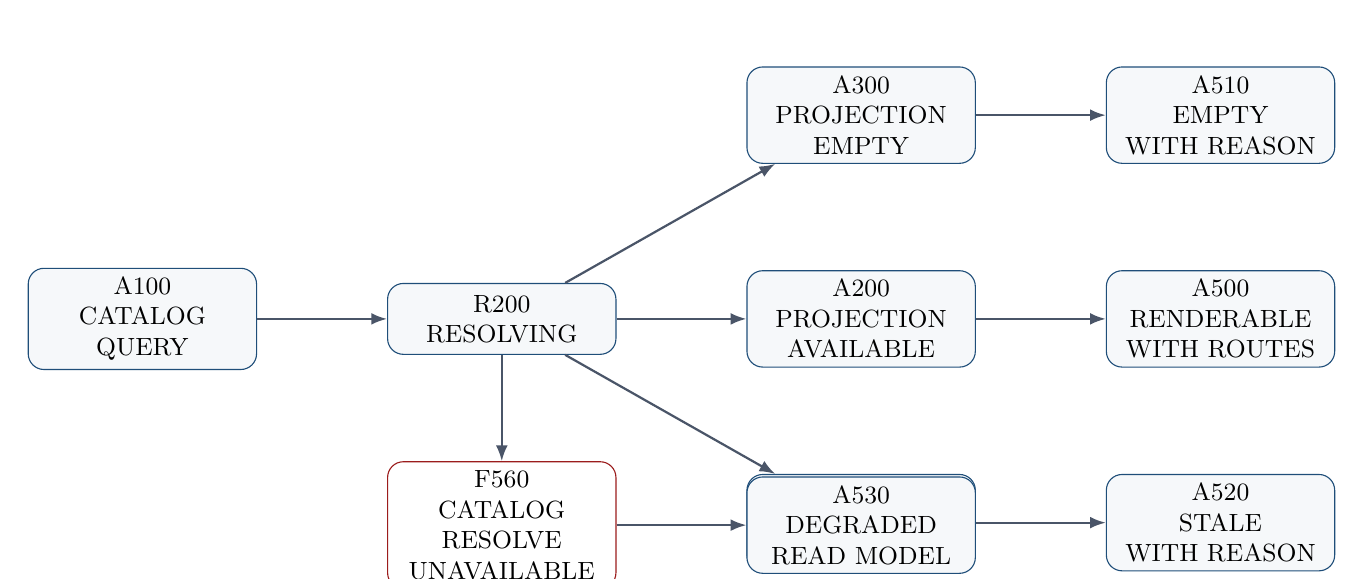
\begin{tikzpicture}[node distance=1.35cm and 1.65cm]
\node[state] (a100) {A100\\CATALOG\\QUERY};
\node[state,right=of a100] (r200) {R200\\RESOLVING};
\node[state,right=of r200] (a200) {A200\\PROJECTION\\AVAILABLE};
\node[state,above=of a200] (a300) {A300\\PROJECTION\\EMPTY};
\node[state,below=of a200] (a400) {A400\\PROJECTION\\STALE};
\node[fail,below=of r200] (f560) {F560\\CATALOG\\RESOLVE\\UNAVAILABLE};
\node[state,right=of a200] (a500) {A500\\RENDERABLE\\WITH ROUTES};
\node[state,right=of a300] (a510) {A510\\EMPTY\\WITH REASON};
\node[state,right=of a400] (a520) {A520\\STALE\\WITH REASON};
\node[state,right=of f560] (a530) {A530\\DEGRADED\\READ MODEL};
\draw[edge] (a100) -- (r200);
\draw[edge] (r200) -- (a200);
\draw[edge] (r200) -- (a300);
\draw[edge] (r200) -- (a400);
\draw[edge] (r200) -- (f560);
\draw[edge] (a200) -- (a500);
\draw[edge] (a300) -- (a510);
\draw[edge] (a400) -- (a520);
\draw[edge] (f560) -- (a530);
\end{tikzpicture}
}
\end{center}

\begin{longtable}{L{0.28\linewidth} L{0.62\linewidth}}
\toprule
Rule & Requirement \\
\midrule
Catalog authority & device-local namespace authority; Hub stores signed projection/read model \\
Backend source & typed \code{ResolveAnswer.records}, not host placement inference \\
Frontend source & API \code{routes[]} and \code{resolve\_unavailable[]}, not local route construction \\
Empty list & only healthy when resolver returns positive empty or typed \code{NODATA} \\
Failure & \code{resolve\_unavailable[]} must be populated for runtime/transport/negative failure \\
\bottomrule
\end{longtable}

\section{Failure Propagation 状态机器}

\begin{center}
\resizebox{\linewidth}{!}{
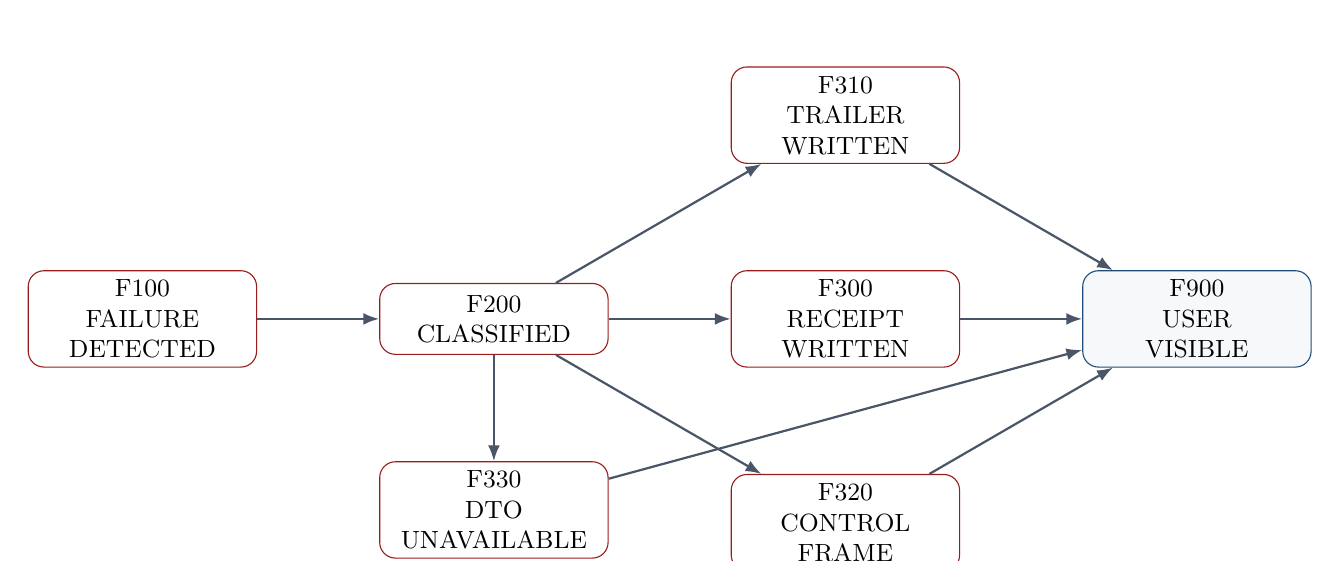
\begin{tikzpicture}[node distance=1.35cm and 1.55cm]
\node[fail] (f100) {F100\\FAILURE\\DETECTED};
\node[fail,right=of f100] (f200) {F200\\CLASSIFIED};
\node[fail,right=of f200] (f300) {F300\\RECEIPT\\WRITTEN};
\node[fail,above=of f300] (f310) {F310\\TRAILER\\WRITTEN};
\node[fail,below=of f300] (f320) {F320\\CONTROL\\FRAME};
\node[fail,below=of f200] (f330) {F330\\DTO\\UNAVAILABLE};
\node[state,right=of f300] (f900) {F900\\USER\\VISIBLE};
\draw[edge] (f100) -- (f200);
\draw[edge] (f200) -- (f300);
\draw[edge] (f200) -- (f310);
\draw[edge] (f200) -- (f320);
\draw[edge] (f200) -- (f330);
\draw[edge] (f300) -- (f900);
\draw[edge] (f310) -- (f900);
\draw[edge] (f320) -- (f900);
\draw[edge] (f330) -- (f900);
\end{tikzpicture}
}
\end{center}

\begin{lstlisting}[language=json,caption={FailureLocator}]
{
  "code": "TARGET_NOT_IN_PRESENCE_REGISTRY",
  "state_code": "F570",
  "source": "daemon_grpc.invoke_remote",
  "layer": "admission",
  "transition": "I300_SUBMITTING -> I400_INVOKING",
  "from_state": "I300_SUBMITTING",
  "interrupted_state": "I400_INVOKING",
  "message": "target device is not in PresenceRegistry",
  "retryable": true,
  "evidence": {
    "target_ura": "easynet:///r/localhost/device/<id>",
    "ability_ura": "easynet:///r/localhost/ability/device.<id>.terminal.list"
  }
}
\end{lstlisting}

\begin{longtable}{L{0.25\linewidth} L{0.25\linewidth} L{0.40\linewidth}}
\toprule
Surface & Failure carrier & Rule \\
\midrule
Unary HTTP before response & JSON \code{\{error,failure\}} & status code may be 4xx/5xx, product reason must be typed \\
HTTP read model & \code{resolve\_unavailable[]} & never return healthy empty list when resolver failed \\
HTTP download after headers & \code{X-EasyNet-Failure} trailer & base64url JSON \code{FailureLocator}, body remains octet-stream \\
WebSocket terminal & \code{terminal\_error} control frame & frontend renders typed code/source/message \\
Invocation receipt & \code{InvocationReceipt.failure} & every Failed/TimedOut/Cancelled receipt writes typed failure \\
\bottomrule
\end{longtable}

\section{核心数据结构}

\subsection{ResolveQuery}

\begin{lstlisting}[language=json]
{
  "target_ura": "easynet:///r/localhost/device/<device-id>",
  "ability_name": "terminal.list",
  "subject_ura": "easynet:///r/localhost/user/<user-id>",
  "caller_ura": "easynet:///r/localhost/user/<user-id>",
  "scope": "TargetOwner",
  "include_abilities": false,
  "release_profile_min": "AuthoritativeLocal"
}
\end{lstlisting}

\subsection{ResolveAnswer.FinalRoute}

\begin{lstlisting}[language=json]
{
  "answer_kind": "FinalRoute",
  "selected_route": {
    "callee_ura": "easynet:///r/localhost/device/<device-id>",
    "ability_ura": "easynet:///r/localhost/ability/device.<device-id>.terminal.list",
    "route_ura": "easynet:///r/localhost/route/<route-id>",
    "dispatch_name": "terminal.list",
    "next_hop": {
      "kind": "LocalDeviceAbility",
      "target_ura": "easynet:///r/localhost/device/<device-id>"
    }
  },
  "route_evidence": {
    "authority": "namespace.resolve",
    "selection_algorithm": "deterministic-weighted",
    "selection_seed_hash": "sha256:...",
    "profile": "Production"
  }
}
\end{lstlisting}

\subsection{Backend Read Model DTO}

\begin{lstlisting}[language=json]
{
  "items": [],
  "routes": [],
  "resolve_unavailable": [
    {
      "source": "namespace.resolve",
      "reason": "NOROUTE",
      "query_name": "terminal.list",
      "message": "target device is not in PresenceRegistry",
      "code": "TARGET_NOT_IN_PRESENCE_REGISTRY",
      "stage": "resolve",
      "retryable": true
    }
  ]
}
\end{lstlisting}

\section{Doctor / Status 输出契约}

\begin{longtable}{L{0.22\linewidth} L{0.68\linewidth}}
\toprule
Field & Required meaning \\
\midrule
\code{state\_code} & stable product state code \\
\code{state} & human-readable state \\
\code{phase} & pairing/join/runtime/namespace/frontend/invoke \\
\code{transition} & last completed or interrupted transition \\
\code{failure.code} & canonical failure code if failed/degraded \\
\code{failure.source} & source component \\
\code{failure.retryable} & operator can retry or must rejoin \\
\code{next\_action} & concrete command or remediation \\
\bottomrule
\end{longtable}

\begin{lstlisting}[caption={doctor human output target}]
EasyNet doctor

  - device pairing       paired as c130295e-9682-499e-bc09-72d4678a5887
  - local runtime        failed
      state_code: F560
      state: BRIDGE_UNAVAILABLE
      transition: S330_DAEMON_BOOTED -> S340_SESSION_ADMITTED
      reason: bridge library not found
      next: set EASYNET_DENDRITE_BRIDGE_LIB or EASYNET_DENDRITE_BRIDGE_HOME, then run easynet runtime start
  - federation           peers configured, namespace not visible
\end{lstlisting}

\section{HTTP / Frontend 状态渲染契约}

\begin{longtable}{L{0.30\linewidth} L{0.15\linewidth} L{0.45\linewidth}}
\toprule
Case & HTTP status & Body rule \\
\midrule
resolver typed negative for list/read model & 200 & rows plus \code{resolve\_unavailable[]}, unless request itself invalid \\
missing canonical ability route in invocation prepare & 400 & typed \code{failure} with \code{R400} or \code{F560}, not bare \code{ability\_ura is required} \\
target offline during invoke & 409/503 & typed \code{failure}, code \code{TARGET\_NOT\_IN\_PRESENCE\_REGISTRY} \\
unauthorized policy & 403 & typed negative \code{UNAUTHORIZED} \\
healthy empty list & 200 & empty rows and no \code{resolve\_unavailable[]} \\
\bottomrule
\end{longtable}

\section{Invocation 全量变体矩阵}

\subsection{维度}

\code{invoke} 不是单一路径, 而是 resolver-selected route 加 transport profile 的组合。完整状态机必须覆盖 locality、tenant boundary 和 transport profile 三个维度。

\begin{longtable}{L{0.20\linewidth} L{0.34\linewidth} L{0.36\linewidth}}
\toprule
Dimension & Values & Contract \\
\midrule
Locality & same device, same realm remote device, cross realm peer, hosted agent, hub/system ability & caller 不能从 locality 推断 route, 必须看 \code{ResolveAnswer.FinalRoute.next\_hop} \\
Tenant boundary & same user, cross user same realm, cross user cross realm, service/system subject & policy result 必须进入 resolve answer 或 admission failure, 不能在 frontend 静默过滤 \\
Transport profile & unary, streaming, bidi, terminal/websocket, download-after-commit, Mission/EAL composite & transport 只能改变 failure carrier, 不能改变 canonical failure shape \\
\bottomrule
\end{longtable}

\subsection{Route variants}

\begin{longtable}{L{0.13\linewidth} L{0.22\linewidth} L{0.20\linewidth} L{0.17\linewidth} L{0.20\linewidth}}
\toprule
Variant & Predicate & Resolver answer & Dispatch next hop & Canonical failures \\
\midrule
\statecode{V0\_LOCAL\_SAME\_DEVICE} & caller、subject、callee 在同一 device runtime & \statecode{FinalRoute(LocalDeviceAbility)} & local ability registry & \statecode{NXDOMAIN}, \statecode{NODATA}, \statecode{UNAUTHORIZED} \\
\statecode{V1\_SAME\_REALM\_SAME\_USER\_REMOTE\_DEVICE} & 同 realm、同 user、目标 device 在线 & \statecode{FinalRoute(RemoteDeviceAbility)} & hub \code{<agent>.invoke\_remote} & \statecode{TARGET\_NOT\_IN\_PRESENCE\_REGISTRY}, \statecode{NOROUTE}, \statecode{STALE} \\
\statecode{V2\_SAME\_REALM\_CROSS\_USER} & 同 realm、跨 user 共享资源或授权 ability & \statecode{FinalRoute} or \statecode{Negative(UNAUTHORIZED)} & hub remote route & \statecode{UNAUTHORIZED}, \statecode{SUBJECT\_KEY\_UNREGISTERED}, \statecode{DELEGATION\_INVALID} \\
\statecode{V3\_CROSS\_REALM} & target realm 与 caller realm 不同 & \statecode{Delegation} then peer \statecode{FinalRoute} & trusted peer hub & \statecode{REALM\_NOT\_TRUSTED}, \statecode{PEER\_HUB\_UNAVAILABLE}, \statecode{DELEGATION\_REQUIRED} \\
\statecode{V4\_HOSTED\_AGENT\_LOCAL\_DEVICE} & ability 属于本机 hosted agent & \statecode{FinalRoute(HostedAgentAbility)} & local agent runtime & \statecode{AGENT\_NOT\_ADVERTISED}, \statecode{AGENT\_NOT\_RUNNING} \\
\statecode{V5\_HOSTED\_AGENT\_REMOTE\_DEVICE} & hosted agent 在远端 device & \statecode{FinalRoute(RemoteHostedAgentAbility)} & hub to owning daemon & \statecode{TARGET\_NOT\_IN\_PRESENCE\_REGISTRY}, \statecode{AGENT\_NOT\_ADVERTISED}, \statecode{OVERLOADED} \\
\statecode{V6\_HUB\_OR\_SYSTEM\_ABILITY} & hub/system-owned ability & \statecode{FinalRoute(HubAbility)} & hub local ability & \statecode{UNAUTHORIZED}, \statecode{ABILITY\_QUERY\_CONFLICT}, \statecode{THROTTLED} \\
\statecode{V7\_BACKEND\_PUBLIC\_RESOURCE} & pages/files/openai 等产品资源 & \statecode{FinalRoute(ProductResourceRoute)} & route-selected host & \statecode{ROUTE\_PROFILE\_NOT\_AUTHORITATIVE}, \statecode{AGENT\_NOT\_ADVERTISED}, \statecode{NOROUTE} \\
\bottomrule
\end{longtable}

\subsection{Transport 子状态机器}

\begin{longtable}{L{0.20\linewidth} L{0.31\linewidth} L{0.22\linewidth} L{0.19\linewidth}}
\toprule
Profile & States & Failure carrier & Rule \\
\midrule
Unary & \code{I100 -> I200 -> I300 -> I410 -> I900/F900} & HTTP JSON or receipt & response 未提交时使用 typed body \\
Server stream & \code{I420 -> I421 -> I422 -> I900/F901} & receipt/control frame & EOF 不能替代 typed close reason \\
Bidi stream & \code{I430 -> I431 -> I432 -> I900/F902} & receipt plus control frame & open failure 和 midstream failure 分开编码 \\
Terminal/WebSocket & \code{I420/I430 -> I421/I431 -> F320/I900} & \code{terminal\_error} frame & frontend 显示 code/source/message \\
Download after commit & \code{D100 -> D200 -> D300 -> I900/D910} & \code{X-EasyNet-Failure} trailer & body 已提交后由 trailer 携带 failure \\
Mission/EAL composite & \code{M100 -> M200 -> M300 -> M900/F910} & parent receipt & child failure 保留, 不 flatten \\
\bottomrule
\end{longtable}

\subsection{Policy matrix}

\begin{longtable}{L{0.26\linewidth} L{0.24\linewidth} L{0.24\linewidth} L{0.18\linewidth}}
\toprule
Caller/subject case & Same realm & Cross realm & Required evidence \\
\midrule
Same user, same device & local positive route & delegation not needed & device credential, session id \\
Same user, remote device & remote positive route if online & peer positive route if trusted & ownership ledger, target presence \\
Cross user, explicit share & positive route only with grant & peer route only with cross-realm grant & grant id, subject URA, caller signature \\
Cross user, no grant & \statecode{Negative(UNAUTHORIZED)} & \statecode{Negative(UNAUTHORIZED)} or \statecode{REALM\_NOT\_TRUSTED} & policy denial evidence \\
System/service caller & system route if role allowed & trusted system delegation & service identity, role proof \\
\bottomrule
\end{longtable}

\section{Stop 状态机器}

\code{runtime stop} 是 operator lifecycle, 不是 unpair。它必须停止本地 daemon/session 并撤销 namespace 可见性, 但保留 credential、trust 和 pairing identity。

\begin{center}
\resizebox{\linewidth}{!}{
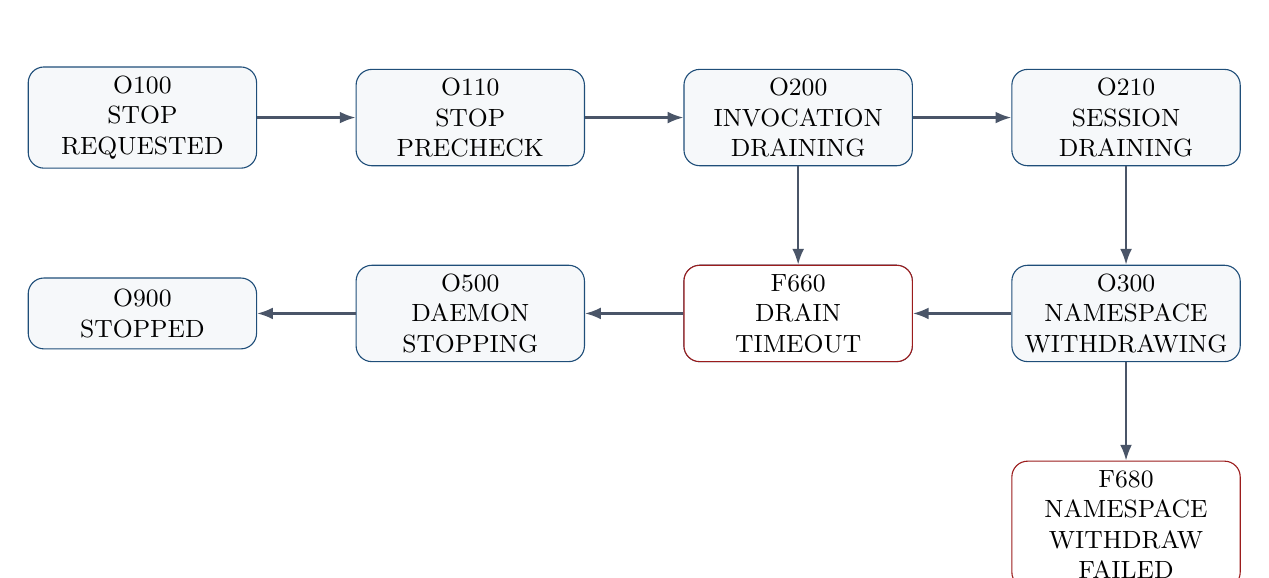
\begin{tikzpicture}[node distance=1.25cm and 1.25cm]
\node[state] (o100) {O100\\STOP\\REQUESTED};
\node[state,right=of o100] (o110) {O110\\STOP\\PRECHECK};
\node[state,right=of o110] (o200) {O200\\INVOCATION\\DRAINING};
\node[state,right=of o200] (o210) {O210\\SESSION\\DRAINING};
\node[state,below=of o210] (o300) {O300\\NAMESPACE\\WITHDRAWING};
\node[state,left=of o300] (o400) {O400\\SESSION\\CLOSING};
\node[state,left=of o400] (o500) {O500\\DAEMON\\STOPPING};
\node[state,left=of o500] (o900) {O900\\STOPPED};
\node[fail,below=of o200] (f660) {F660\\DRAIN\\TIMEOUT};
\node[fail,below=of o300] (f680) {F680\\NAMESPACE\\WITHDRAW\\FAILED};
\draw[edge] (o100) -- (o110);
\draw[edge] (o110) -- (o200);
\draw[edge] (o200) -- (o210);
\draw[edge] (o210) -- (o300);
\draw[edge] (o300) -- (o400);
\draw[edge] (o400) -- (o500);
\draw[edge] (o500) -- (o900);
\draw[edge] (o200) -- (f660);
\draw[edge] (o300) -- (f680);
\end{tikzpicture}
}
\end{center}

\begin{longtable}{L{0.10\linewidth} L{0.25\linewidth} L{0.20\linewidth} L{0.35\linewidth}}
\toprule
Code & State & Owner & Invariant \\
\midrule
\code{O100} & \statecode{STOP\_REQUESTED} & CLI & user requested runtime stop \\
\code{O110} & \statecode{STOP\_PRECHECK} & CLI daemon & load local runtime identity; no network-heavy inference \\
\code{O200} & \statecode{INVOCATION\_DRAINING} & CLI daemon & in-flight invocations get completed/cancelled receipts \\
\code{O210} & \statecode{SESSION\_DRAINING} & CLI daemon / Axon bridge & stop accepting new remote invocations \\
\code{O300} & \statecode{NAMESPACE\_WITHDRAWING} & CLI daemon / Hub & withdraw advertised abilities/presence \\
\code{O400} & \statecode{SESSION\_CLOSING} & CLI daemon / Hub & close admitted session with reason \code{operator\_stop} \\
\code{O500} & \statecode{DAEMON\_STOPPING} & CLI supervisor & daemon process exits or is killed after timeout \\
\code{O900} & \statecode{STOPPED} & CLI & daemon stopped; credential remains \\
\code{F650} & \statecode{STOP\_PRECHECK\_FAILED} & CLI & local runtime identity/config unreadable \\
\code{F660} & \statecode{DRAIN\_TIMEOUT} & CLI daemon & pending receipts must be cancelled \\
\code{F670} & \statecode{SESSION\_CLOSE\_FAILED} & CLI daemon / Hub & local stop may continue but state is degraded \\
\code{F680} & \statecode{NAMESPACE\_WITHDRAW\_FAILED} & CLI daemon / Hub & namespace visibility may be stale \\
\code{F690} & \statecode{DAEMON\_STOP\_FAILED} & CLI supervisor & process did not stop \\
\bottomrule
\end{longtable}

\section{Self Uninstall / Leave 状态机器}

\code{self uninstall}/\code{leave} 是 identity lifecycle。它撤销本地 device identity、trust material、cached projections 和 backend pairing, 与 \code{runtime stop} 不同。clean target 不兼容旧的静默清理: 部分失败必须可见且可恢复。

\begin{longtable}{L{0.10\linewidth} L{0.27\linewidth} L{0.18\linewidth} L{0.35\linewidth}}
\toprule
Code & State & Owner & Invariant \\
\midrule
\code{U100} & \statecode{UNINSTALL\_REQUESTED} & CLI & explicit destructive user request \\
\code{U110} & \statecode{IDENTITY\_LOADED} & CLI & load device id, realm, credential paths, trust paths \\
\code{U200} & \statecode{LOCAL\_RUNTIME\_STOPPING} & CLI & reuse stop state machine; no live session may remain advertised \\
\code{U300} & \statecode{NAMESPACE\_REVOKING} & CLI daemon / Hub & remove presence/ability advertisements and revoke namespace authority \\
\code{U400} & \statecode{BACKEND\_PAIRING\_REVOKING} & Backend & mark device pairing revoked/removed with typed reason \\
\code{U500} & \statecode{LOCAL\_CREDENTIALS\_REMOVING} & CLI & delete device credential/private local config \\
\code{U600} & \statecode{TRUST\_REMOVING} & CLI & remove realm trust files only if no other identity needs them \\
\code{U700} & \statecode{LOCAL\_CACHE\_PURGING} & CLI & purge read model/session/invocation cache for this identity \\
\code{U900} & \statecode{UNINSTALLED} & CLI / Backend & local identity cannot invoke; frontend shows removed/unpaired \\
\code{F710} & \statecode{IDENTITY\_NOT\_FOUND} & CLI & visible unless user requested allow-missing \\
\code{F720} & \statecode{UNINSTALL\_STOP\_FAILED} & CLI & do not delete credentials while runtime may still advertise \\
\code{F730} & \statecode{REVOKE\_FAILED\_RETRYABLE} & CLI / Hub & backend/hub revoke failed; pause or mark partial \\
\code{F740} & \statecode{CREDENTIAL\_REMOVE\_FAILED} & CLI & local credential deletion failed \\
\code{F750} & \statecode{TRUST\_REMOVE\_FAILED} & CLI & trust cleanup failed \\
\code{F760} & \statecode{CACHE\_PURGE\_FAILED} & CLI & cache cleanup failed, identity already revoked \\
\code{F770} & \statecode{PARTIAL\_UNINSTALL} & CLI / Backend & irreversible steps completed; doctor shows remaining cleanup \\
\bottomrule
\end{longtable}

\section{Canonical Failure Code Catalog}

\noindent\textbf{Pairing/join/runtime}\\
Codes: \statecode{PAIRING\_TOKEN\_EXPIRED}, \statecode{PAIRING\_TOKEN\_CONSUMED}, \statecode{HUB\_UNREACHABLE}, \statecode{CREDENTIAL\_REJECTED}, \statecode{DAEMON\_BOOT\_FAILED}, \statecode{BRIDGE\_LIBRARY\_NOT\_FOUND}, \statecode{SESSION\_ADMISSION\_REJECTED}, \statecode{NAMESPACE\_NOT\_VISIBLE}.\\
Surfaces: join, doctor, backend device DTO.

\noindent\textbf{Resolver negative}\\
Codes: \statecode{ABILITY\_QUERY\_CONFLICT}, \statecode{NXDOMAIN}, \statecode{NODATA}, \statecode{NOROUTE}, \statecode{UNAUTHORIZED}, \statecode{STALE}, \statecode{THROTTLED}, \statecode{OVERLOADED}, \statecode{ROUTE\_PROFILE\_NOT\_AUTHORITATIVE}.\\
Surfaces: resolve answer, read model DTO.

\noindent\textbf{Routing/tenant}\\
Codes: \statecode{REALM\_NOT\_TRUSTED}, \statecode{PEER\_HUB\_UNAVAILABLE}, \statecode{DELEGATION\_REQUIRED}, \statecode{DELEGATION\_INVALID}, \statecode{SUBJECT\_KEY\_UNREGISTERED}, \statecode{CALLER\_SIGNATURE\_INVALID}, \statecode{TARGET\_NOT\_IN\_PRESENCE\_REGISTRY}, \statecode{AGENT\_NOT\_ADVERTISED}, \statecode{AGENT\_NOT\_RUNNING}.\\
Surfaces: resolver answer, invocation receipt.

\noindent\textbf{Invocation transport}\\
Codes: \statecode{STREAM\_OPEN\_FAILED}, \statecode{STREAM\_CLOSED}, \statecode{BIDI\_OPEN\_FAILED}, \statecode{DOWNLOAD\_TRAILER\_FAILURE}, \statecode{RECEIPT\_FAILURE\_MISSING}, \statecode{CHILD\_INVOCATION\_FAILED}.\\
Surfaces: receipt, trailer, WebSocket/control frame.

\noindent\textbf{Stop lifecycle}\\
Codes: \statecode{STOP\_PRECHECK\_FAILED}, \statecode{DRAIN\_TIMEOUT}, \statecode{SESSION\_CLOSE\_FAILED}, \statecode{NAMESPACE\_WITHDRAW\_FAILED}, \statecode{DAEMON\_STOP\_FAILED}.\\
Surfaces: \code{runtime stop}, \code{doctor --json}.

\noindent\textbf{Self-uninstall lifecycle}\\
Codes: \statecode{IDENTITY\_NOT\_FOUND}, \statecode{UNINSTALL\_STOP\_FAILED}, \statecode{REVOKE\_FAILED\_RETRYABLE}, \statecode{CREDENTIAL\_REMOVE\_FAILED}, \statecode{TRUST\_REMOVE\_FAILED}, \statecode{CACHE\_PURGE\_FAILED}, \statecode{PARTIAL\_UNINSTALL}.\\
Surfaces: \code{self uninstall}/\code{leave}, \code{doctor --json}.

\begin{decisionbox}
Failure code 与状态码不是同一个字段: 状态码定位 state/transition, failure code 解释协议或产品原因。例如 \code{F900 INVOCATION\_FAILED} 可以携带 \statecode{TARGET\_NOT\_IN\_PRESENCE\_REGISTRY}、\statecode{UNAUTHORIZED} 或 \statecode{AGENT\_NOT\_ADVERTISED}。
\end{decisionbox}

\section{治本更新计划}

\begin{enumerate}[leftmargin=*]
  \item \textbf{Axon contract finalization}: \code{ResolveAnswer} 成为唯一 route wire/product contract; \code{Negative} 覆盖 deterministic taxonomy; \code{InvocationReceipt.failure} 覆盖 Failed/TimedOut/Cancelled。
  \item \textbf{CLI daemon resolve-before-invoke}: 所有 local/remote invoke path 先 \code{namespace.resolve}; dispatch 只消费 resolver-selected next hop; doctor 输出 connection snapshot 和 interrupted transition。
  \item \textbf{Backend route facade cleanup}: prepare envelope 调 daemon \code{namespace.resolve}; 删除长期 \code{canonicalDeviceAbilityRoute} 和 owner inference fallback; \code{history/list} 返回 typed route failure。
  \item \textbf{Backend read model typed unavailable}: devices、abilities、agents、skills、pages、calls、history 全部保留 \code{resolve\_unavailable[]}。
  \item \textbf{Frontend route source cleanup}: ability action 按 API \code{routes[]} 或 selected route id 调用; 下载 client 解码 \code{X-EasyNet-Failure} trailer。
  \item \textbf{Receipt producer consolidation}: terminal/file/browser/remote desktop/openai pages 等 producer 统一写 \code{InvocationReceipt.failure}。
  \item \textbf{End-to-end gates}: docker compose 内覆盖 bridge missing、hub offline、target offline、agent not advertised、unauthorized 五类失败。
  \item \textbf{Operator lifecycle gates}: \code{runtime stop} 使用 \code{O*} 状态机; \code{self uninstall}/\code{leave} 使用 \code{U*} 状态机; \code{doctor --json} 在 join、invoke、stop、uninstall 中输出同构状态对象: \code{state\_code}, \code{failure}, \code{transition}, \code{next\_action}。
\end{enumerate}

\section{剩余任务清单}

\begin{longtable}{L{0.10\linewidth} L{0.46\linewidth} L{0.22\linewidth} L{0.14\linewidth}}
\toprule
Priority & Task & Owner repo & Target state \\
\midrule
P0 & CLI daemon 所有 invoke path 统一 resolve-before-invoke & EasyNet-Cli & \code{R200 -> R300 -> I400} \\
P0 & Backend prepare/submit 删除 canonical ability inference & EasyNet Backend & \code{R300 -> I100} \\
P0 & \code{invocations/history/list} 改为 resolver catalog route 或 typed failure & Backend/Frontend & no bare 400 \\
P0 & \code{meta.list\_resources} 选择 resolver catalog route & CLI/Backend & no missing route \\
P1 & Frontend 全部 ability action 消费 \code{routes[]} & Frontend & no owner inference \\
P1 & 下载 client 解码 \code{X-EasyNet-Failure} trailer & Frontend & typed download failure \\
P1 & 所有 terminal receipt producer 写 \code{InvocationReceipt.failure} & CLI/Axon & typed receipt \\
P1 & \code{runtime stop} 输出 \code{O*} 状态码和 interrupted transition & EasyNet-Cli & stop traceable \\
P1 & \code{self uninstall/leave} 输出 \code{U*} 状态码和 partial cleanup & CLI/Backend & uninstall traceable \\
P1 & invoke 变体按 route/transport profile 写 fixture & Axon/CLI & complete invoke matrix \\
P2 & RFC-005 failure code taxonomy 细化 & Axon & fewer generic failures \\
P2 & Docker e2e 增加 five-failure matrix & all & regression gate \\
\bottomrule
\end{longtable}

\section{验收矩阵}

\begin{longtable}{L{0.45\linewidth} L{0.30\linewidth} L{0.17\linewidth}}
\toprule
Scenario & Expected state & Expected code \\
\midrule
token expired before CLI validate & \statecode{PAIRING\_TOKEN\_EXPIRED} & \code{F120} \\
join saved credential but Hub TLS unreachable & \statecode{HUB\_UNREACHABLE} & \code{F530} \\
bridge library missing & \statecode{BRIDGE\_UNAVAILABLE} & \code{F560} \\
daemon up but session admission rejected & \statecode{SESSION\_ADMISSION\_REJECTED} & \code{F570} \\
device not in PresenceRegistry on \code{terminal.list} & \statecode{ROUTE\_NEGATIVE} or degraded read model & \statecode{TARGET\_NOT\_IN\_PRESENCE\_REGISTRY} \\
pages agent not advertised & degraded pages read model & \statecode{AGENT\_NOT\_ADVERTISED} \\
history/list lacks selected route & typed prepare failure & \statecode{ABILITY\_ROUTE\_REQUIRED} or \code{NOROUTE} \\
healthy empty pages & render empty with no unavailable & no failure \\
failed terminal invocation & receipt failure populated & canonical failure code \\
cross realm untrusted invoke & \statecode{ROUTE\_NEGATIVE} & \statecode{REALM\_NOT\_TRUSTED} \\
same realm cross-user without grant & \statecode{ROUTE\_NEGATIVE} & \statecode{UNAUTHORIZED} \\
runtime stop success & \statecode{STOPPED} & \code{O900} \\
runtime stop drain timeout & \statecode{DRAIN\_TIMEOUT} & \code{F660} \\
self uninstall partial backend revoke failure & \statecode{PARTIAL\_UNINSTALL} & \code{F770} \\
\bottomrule
\end{longtable}

\section{工程对象边界}

\begin{decisionbox}
\tagderived{} 干净实现不应通过堆叠 if/else 消灭症状, 而应把状态机、resolver facade、catalog route DTO、failure locator 和 receipt mapper 分成职责小而硬的对象。
\end{decisionbox}

{\raggedright
\noindent{\statecode{ConnectionStateMachine}}\\
CLI-owned local join/runtime/namespace snapshot; 决定状态和 transition, 不做 IO。

\noindent{\statecode{ResolveRouteFacade}}\\
Backend-owned product facade over daemon \code{namespace.resolve}; 只返回 typed route/negative/unavailable。

\noindent{\statecode{AbilityCatalogRoute}}\\
Backend/Frontend shared DTO route item; UI action 的唯一 route source。

\noindent{\statecode{FailureLocator}}\\
Axon/CLI/Backend shared failure projection; carrier 可随 transport 变化。

\noindent{\statecode{InvocationReceiptFailureMapper}}\\
runtime producer mapper; transport/runtime/admission errors 到 canonical receipt failure。
\par}

\end{document}
